\documentclass{acm}
\usepackage{graphicx}
\usepackage{mathptmx}
\usepackage{fixltx2e}
\usepackage[hidelinks]{hyperref}
\usepackage{multirow} 
\usepackage{float}
\usepackage{amsfonts}
\usepackage{color}
\usepackage{soul}
\newcommand{\TODO}[1]{\hl{TODO: #1}}


%\usepackage{times}
%\normalfont
%\usepackage[T1]{fontenc}
%\usepackage[mtplusscr,mtbold]{mathtime}
\begin{document}

\title{Yarncraft: Location Aware Narratives in Virtual Space}

\numberofauthors{3}
\author{
\alignauthor
Tom Blount\\
	   \affaddr{Web and Internet Science}\\
       \affaddr{Electronics and Computer Science}\\
       \affaddr{University of Southampton}\\
       \affaddr{Southampton, United Kingdom}\\
       \email{tb12g09@ecs.soton.ac.uk}
% 2nd. author
\alignauthor
Jonathan Scott\\
       \affaddr{Web and Internet Science}\\
       \affaddr{Electronics and Computer Science}\\
       \affaddr{University of Southampton}\\
       \affaddr{Southampton, United Kingdom}\\
       \email{js3g10@ecs.soton.ac.uk}
% 3rd. author
\alignauthor
David E. Millard\\
       \affaddr{Web and Internet Science}\\
       \affaddr{Electronics and Computer Science}\\
       \affaddr{University of Southampton}\\
       \affaddr{Southampton, United Kingdom}\\
       \email{dem@ecs.soton.ac.uk}
% 4th. author
%\alignauthor
%Mark J. Weal\\
%       \affaddr{Web and Internet Science}\\
%       \affaddr{Electronics and Computer Science}\\
%       \affaddr{University of Southampton}\\
%       \affaddr{Southampton, United Kingdom}\\
%       \email{mjw@ecs.soton.ac.uk}
}
\date{July 2016}

\permission{Permission to make digital or hard copies of all or part of this work for personal or classroom use is granted without fee provided that copies are not made or distributed for profit or commercial advantage and that copies bear this notice and the full citation on the first page. Copyrights for components of this work owned by others than ACM must be honored. Abstracting with credit is permitted. To copy otherwise, or republish, to post on servers or to redistribute to lists, requires prior specific permission and/or a fee. Request permissions from Permissions@acm.org.}
\conferenceinfo{NHT '16}{July 10 2016, Dalhousie University, Halifax, Nova Scotia}

\copyrightetc{\the\acmcopyr}
\crdata{\copyright 2016 ACM. ISBN XXX-X-XXXX-XXXX-X/XX/XX...\$15.00.\\
DOI: http://xxxxxxxxxxxxxxxxxxxxxxx}

\maketitle
\begin{abstract}
\TODO{ABSTRACT}
\end{abstract}

\category{H.1}{Models and Principles} General

\keywords{narrative; location-aware; virtual spaces; virtual worlds;}

\section{Introduction}
\TODO{What's the problem?}

\TODO{Why's it a problem?}

\TODO{How've we fixed it?}


\section{Background}
Hypertextual narratives are digital narratives that do not necessarily need to be read in a linear order and may branch in multiple places, allowing for many different tellings and re-tellings. A location-aware hypertextual narrative can detect the reader's position in space (through, for example, their mobile phone's GPS), allowing an author to guide a user around a specific set of locations with which they use to tell their story. Linking a narrarative to the reader's physical location can provide readers with a more immersive experience \cite{karapanos2012does}. Location-aware narratives have been developed to aid education and learning by providing an engaging link between practice and theory \cite{ardito2007mobile, rogers2005ubi}, to create interactive games \cite{benford2003coping, bunting2012player} and simply to tell stories about a particular location \cite{dionisio2010iland, pittarello2011designing}

Virtual social worlds (and virtual game worlds) are computer-simulated environments in which users can interact with one another and the environment itself \cite{Kaplan2010}. These virtual spaces are a growing way in which people can meet both socially \cite{kaplan2009fairyland}, recreationally \cite{wu2008they} and even for business applications \cite{erickson2011synchronous}. 

Virtual social worlds have also been used in the context of presenting a novel way of telling narratives, with applications such as
\TODO{Background}
games
augmented reality
learning tools \cite{avouris2012review}

As such, there is a clear overlap in the use-cases of location-aware narratives and virtual worlds.

Millard et al. have proposed a model of sculptural hypertext, suitable for location-aware narratives, that links existing theory with observable structures of hypertext, and opens the possibility of moving towards a standardised format for viewers and authoring tools \cite{millard13canyons}. This model consists of three structures -- canyons, deltas and plains -- that can be combined to represent all possible patterns of location-aware narrative. These three structures are built up of atomic ``cards'' or ``pages'' in different orientations. In canyons, they form a linear sequence with transitions from one page to another; in deltas they form a branching sequence in which each page can link to multiple pages; and in plains they remain ``floating'' unconnected, and can be accessed in any order the reader chooses. Constraints (such as being read in a particular order, being read at a particular time, or being read in a particular location) can be imposed on these structures to build more complex structures.


\section{Yarncraft}

Yarncraft is an attempt to leverage Millard et al.'s location-aware model of sculptural hypertext and in particular to adapt the framework of the GeoYarn client they developed to allow arbitrary narratives to be traversed in either physical or virtual space.

For our example, we tailor one of the stories marked up in their framework for use in a physical space around the city of Southampton to be used instead in Minecraft\footnote{http://minecraft.net/}, a creative sandbox virtual world that allows players to explore a stylised, procedurally-generated environment, build structures and artwork, and interact with friendly and hostile non-player characters (NPCs).

This was a two-stage process -- firstly, tailoring the framework to be suitable for virtual locations in general (and particularly for use within Minecraft) and secondly, developing a mod to Minecraft to allow it to read the framework and present the narrative to the user.

The interface to the Minecraft mod is, at this stage, relatively simplistic, and the : the user is present

\begin{figure}
\centering
\begin{verbatim}
"locations": [
             	{
                		"type": "NearbyLocation",
                        "nearby": "Water",
                        "distance": 5
                }
]
\end{verbatim}

\caption{``Suddenly, a crowd appeared''}
\label{figure:villagers}
\end{figure}


Millard et al.'s framework allows for two types of locations to be used: precise locations, that map to specific areas defined by latitude and longitude points, and abstract locations that are defined by adjectives such as ``quiet'', ``green'' or ``crowded''.

With virtual worlds, even deeper information about the user and their virtual surroundings can be gathered without additional sensor hardware (as long as it is exposed by the appropriate API), such as the weather, light level or noise level.
further abstract context and statistics such as


Location-aware narratives based in the physical world allow the story to be adapted to the user's location either through branching the story as the user moves through space, or by modifying the tone of a page to suit the user's current location. However, with a virtual world, the world itself can also be adapted as the narrative progresses. This can be done to shape the general aesthetic and environment of the virtual world to be in keeping with the narrative (as a whole, or at a specific point in time); for example, altering the weather or light levels.  This can also be leveraged if the author wishes to trigger specific events during the course of the story. In Figure \ref{figure:gather} the player is instructed to go to a place where people gather. Due to the state of mind of the protagonist of the story, it appears deserted at first. But, when the player arrives in Figure \ref{figure:villagers}, a crowd of friendly NPC villagers appear around them.

\begin{figure}
\centering
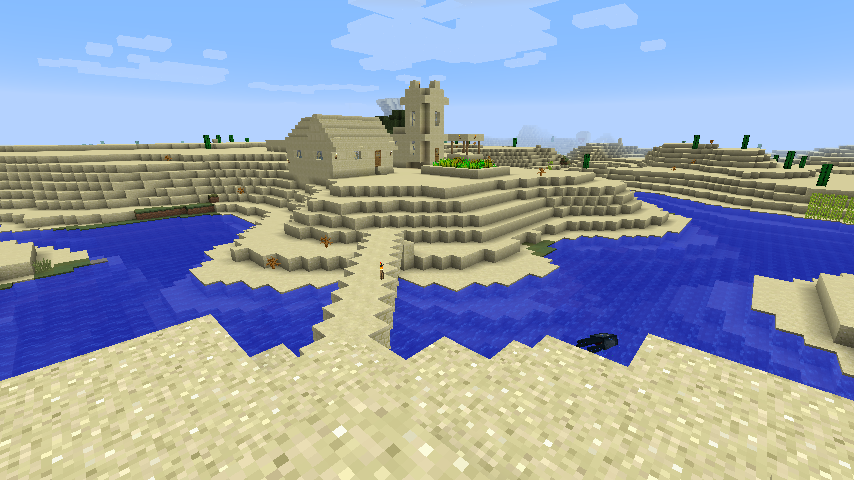
\includegraphics[scale=.24]{./figures/place.png}
\caption{``A place where people gather''}
\label{figure:gather}
\end{figure}

\begin{figure}
\centering
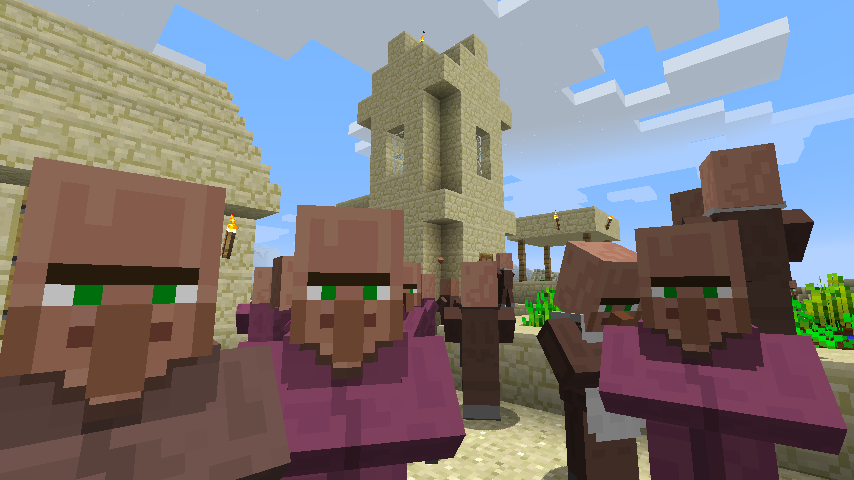
\includegraphics[scale=0.24]{./figures/villagers.png}
\caption{``Suddenly, a crowd appeared''}
\label{figure:villagers}
\end{figure}


\section{Discussion}
\TODO{Abstracting}
Fine balance between abstracting the framework enough that it can be generally applied to other virtual spaces, and 


\TODO{Manipulating environment}
However, while this can lead to a more tailored (and potentially immersive) experience, the greater and more specific the degree of control exerted over the virtual world, the less abstract the framework becomes.

One initial drawback with this approach is that each virtual world will require a specific plug-in to read the story framework, 

While this does create an initial barrier to entry for authors trying to develop stories for unsupported platforms, once a plug-in is developed it can be reused for multiple individual stories.

\TODO{Future work}
\TODO{Adapting the client?}
\TODO{User marked locations}
One issue faced by location-aware narratives, both physical and virtual, is the possibility that there may be no appropriate locations, such as a bar, in the nearby vicinity. However, virtual spaces face this problem, but a further step removed: the concept  of a drinking establishment may not even exist in a particular virtual world. One possible means of remedying this would be to, once the client loads and parses the story, to present the user with a map of their virtual space and ask them to self-define areas for use in the story, or simply allowing them to ``spoof'' their location on-the-fly, to proceed with the next part of the story.

\TODO{Demonstrating multiple platforms}
\TODO{More science}
Another interesting avenue for future work is to investigate whether readers still feel the extra immersion in a virtual world they feel ``at home'' in (such as a Minecraft world that they have spend time and effort building in) when compared to the physical world, or a virtual world they have no previous attachment to.

\section{Conclusions}
\TODO{Conclusions}

\bibliographystyle{abbrv}
\bibliography{library}
%\begin{thebibliography}{26}
%\end{thebibliography}

\end{document}
